
% 微分方程的数值方法

\chapter{EM数值方法}

\section{假设和引理}
\begin{assumption}\label{Lipschitz}
	在这一章节中, 我们假设SDE\cref{basic SDE}的漂移项系数$f$满足全局\textnormal{Lipschitz}条件的, 即存在一个常数$K>0$, 使得:
	\begin{equation}
		|f(x)-f(y)| \le K|x-y|. 
	\end{equation}
\end{assumption}

\begin{assumption}\label{linear growth}
	在这一章节中, 我们假设SDE\cref{basic SDE}的漂移项系数$f$满足线性增长条件, 即存在一个常数$K>0$, 使得:
	\begin{equation}
		|f(x)| \le K(1+|x|). 
	\end{equation}
\end{assumption}

\section{强收敛性}
\begin{proposition}\label{main pro}
	令X是SDE\cref{basic SDE}的解, 其中f满足\cref{moment}, \cref{Lipschitz}和\cref{linear growth}, 那么对于任意的$p \ge 1$, 都有$\mathbb{E}[Y_T^{(p)}] < \infty$, 其中$Y_t^{(p)} := 1 + \sup\limits_{0\le r\le t}|X_r|^p$.
\end{proposition}
\begin{proof}
	设 $S_{\ell} := \inf\{ t \geq 0 : Y_{t}^{(p)} > \ell \}$,其中 $\ell \in \mathbb{N}$。由于解 $X$ 具有连续的路径,对每个 $t \geq 0$,$Y_{t}^{(p)} < \infty$,因此,随着 $\ell \to \infty$,$S_{\ell} \uparrow \infty$。对于 $\mathbb{P}_D$ 几乎处处的路径,我们首先将 Gronwall 型不等式应用于函数 $t \mapsto \mathbb{E}_B[Y_{t \wedge S_{\ell}}^{(p)}]$ 对于固定的 $\ell$,然后令 $t = T$ 并在得到的不等式中让 $\ell \to \infty$ 来建立 $\mathbb{E}_B[Y_T^{(p)}]$ 的上界。请注意,由于 $S_{\ell}$ 的定义,
	\[
	\int_{0}^{t} \mathbb{E}_B[Y_{r \wedge S_{\ell}}^{(p)}] \, dE_r \leq \ell E_t < \infty,
	\]
	这使得我们可以安全地应用 Gronwall 型不等式。
	
	假设 $p \geq 2$,因为对于 $1 \leq p < 2$ 的结果可以直接通过应用 $p \geq 2$ 时的结果和 Jensen 不等式得到。根据时间变换的Itô 公式,有 $X_s^p = x_0^p + J_s + K_s$,其中
	\[
	J_s := \int_0^s \sigma p X_r^{p-1}  \, dB_{E_r};
	\]
	\[
	K_s := \int_0^s \left\{ p X_r^{p-1} f(X_r) + \frac{\sigma^2}{2} p (p-1) X_r^{p-2}  \right\} \, dE_r.
	\]
	固定 $t \in [0, T]$ 和 $\ell \in \mathbb{N}$。根据\cref{linear growth} 以及不等式 $(x + y + z)^p \leq c_p (x^p + y^p + z^p)$,其中 $x, y, z \geq 0$ 且 $c_p = 3^{p-1}$,有
	\[
	\mathbb{E}_B\left[ \sup_{0 \leq s \leq t \wedge S_{\ell}} |K_s| \right] \leq \left( p c_p K + \frac{1}{2} p(p-1) c_p K^2 \right) \int_0^{t \wedge S_{\ell}} \mathbb{E}_B[Y_r^{(p)}] \, dE_r.
	\]
	由于 $(J_s)_{s \geq 0}$ 是一个局部鞅,应用 BDG 不等式得到
	\[
	\mathbb{E}_B\left[\sup_{0 \leq s \leq t \wedge S_{\ell}} |J_s| \right] \leq b_1 \mathbb{E}_B \left[\left( \int_0^{t \wedge S_{\ell}} \sigma^2 p^2 X_r^{2p-2}  \, dE_r \right)^{1/2}\right],
	\]
	因此,
	\[
	\mathbb{E}_B \left[\sup_{0 \leq s \leq t \wedge S_{\ell}} |J_s| \right] \leq b_1 \mathbb{E}_B \left[ p c_p K \left( Y_{t \wedge S_{\ell}}^{(p)} \int_0^{t \wedge S_{\ell}} Y_r^{(p)} \, dE_r \right)^{1/2} \right]
	\]
	\[
	\leq \frac{1}{2} \mathbb{E}_B \left[Y_{t \wedge S_{\ell}}^{(p)}\right] + 2b_1^2 p^2 c_p^2 K^2 \int_0^{t \wedge S_{\ell}} \mathbb{E}_B \left[Y_r^{(p)}\right] \, dE_r,
	\]
	其中最后一个不等式由基本不等式 $(ab)^{1/2} \leq a/\lambda + \lambda b$ 导出,适用于任意 $a, b, \lambda > 0$,且 $\lambda := 2b_1 p c_p K$. 
	注意,对于任意非负过程 $(L_t)_{t \geq 0}$,都有
	\[
	\int_0^{t \wedge S_{\ell}} L_r \, dE_r \leq \int_0^t L_{r \wedge S_{\ell}} \, dE_r.
	\]
	确实,当 $t \leq S_{\ell}$ 时,不等式显然成立,而如果 $t > S_{\ell}$,则
	\[
	\int_0^{S_{\ell}} L_r \, dE_r + \int_{S_{\ell}}^t L_{S_{\ell}} \, dE_r \geq \int_0^{t \wedge S_{\ell}} L_r \, dE_r.
	\]
	因此,通过上面对 $J_s$ 和 $K_s$ 的估计,有
	\[
	\mathbb{E}_B[Y_{t \wedge S_{\ell}}^{(p)}] \leq 2(1 + |x_0|^p) + 2K^2\left(p c_p K + \left(p(p-1) c_p / 2 + 2b_1^2 p^2 c_p^2\right) \right)\int_0^t \mathbb{E}_B[Y_{r \wedge S_{\ell}}^{(p)}] \, dE_r,
	\]
	通过应用Gronwall 型不等式,得到
	\[
	\mathbb{E}_B[Y_{t \wedge S_{\ell}}^{(p)}] \leq 2(1 + |x_0|^p) e^{2K^2E_T\left(p c_p K + \left(p(p-1) c_p / 2 + 2b_1^2 p^2 c_p^2\right) \right) }.
	\]
	令 $t = T$,并让 $\ell \to \infty$,由于 $\xi(u)$ 不依赖于 $\ell$,并应用单调收敛定理,可得
	\[
	\mathbb{E}_B[Y_T^{(p)}] \leq 2(1 + |x_0|^p) e^{2K^2E_T \left(p c_p K + \left(p(p-1) c_p / 2 + 2b_1^2 p^2 c_p^2\right) \right)}. 
	\]
	对两边取期望$\mathbb{E}_D$, 得到 $\mathbb{E}[Y_T^{(p)}] \leq \mathbb{E}[ce^{cE_T}] < \infty$,这归因于 \cite{jin2019strong}中定理 1的结果。
	
	
	
\end{proof}

\begin{theorem}\label{main th EM}
	对于任意的$\epsilon>0$, 令$\epsilon < T_1 < T_2$, 在\textnormal{\cref{moment}}, \textnormal{\cref{Lipschitz}}和\cref{linear growth}的条件下, 存在常数C, 使得下面的不等式成立:
	$$\mathbb{E}\left[\sup\limits_{i=\lceil T_1/\Delta t \rceil\ldots \lceil T_2/\Delta t \rceil } |X({t_i})-X_{t_i}|\right]\le C\Delta t^\alpha$$
\end{theorem}
\begin{proof}
	
	考虑SDE \eqref{basic SDE}在$[t_i, t_{i+1})$的积分:
	\begin{align}
		\int_{t_i}^{t_{i+1}}dX(s)=\int_{t_i}^{t_{i+1}}f(X(s))dE(s)+\int_{t_i}^{t_{i+1}}\sigma dB(E(s)). 
	\end{align}
	由时间变换的变量变换公式\cite{kobayashi2011stochastic}, 上式等价于
	\begin{align}\label{eq:SDE1}
		\int_{t_i}^{t_{i+1}}dX(s))=\int_{E_{t_i}}^{E_{t_{i+1}}}f(X(D(s-)))ds+\int_{t_i}^{t_{i+1}}\sigma dB(E(s)). 
	\end{align}
	针对于漂移项$f(X(D(s-)))$, 下面等式恒成立:
	\begin{align}\label{eq:ito}
		\int_{E(t_i)}^{E(t_{i+1})} f(X(D(t-)))) - f(X(D(t_i-))) dt = \int_{E(t_i)}^{E(t_{i+1})} \int^{D(t-)}_{D(t_i-)} df(X(s)) dt. 
	\end{align}
	由\cref{ito}的时间变换It\^{o}公式, 于是\eqref{eq:ito}变成
	\begin{equation}\label{eq:ito1}
		\begin{aligned}
			&\quad\int_{E(t_i)}^{E(t_{i+1})} f(X(D(t-))) - f(X(D(t_i-))) dt \\
			&= \int_{E(t_i)}^{E(t_{i+1})} \int_{t_i}^{t} \left( f(X(D(s-))) f^{\prime}(X(D(s-))) + \frac{1}{2} \sigma^2 f^{\prime\prime}(X(D(s-))) \right) ds \, dt\\
			&\quad + \int_{E(t_i)}^{E(t_{i+1})} \int_{t_i}^{t} \sigma f^{\prime}(X(D(s-))) \, dB(s) \, dt . 
		\end{aligned}
	\end{equation}
	由\eqref{eq:SDE1}与\eqref{eq:ito1}, 以及时间变换的变量变换公式可以得到
	\begin{align*}
		X(t_{i+1}) 
		&= X(t_i) + \int_{E(t_i)}^{E(t_{i+1})} f(X({D(t_i-)})) \, dt + \int_{t_i}^{t_{i+1}} \sigma \, dB(E(t)) \\
		&\quad + \int_{E(t_i)}^{E(t_{i+1})} \int_{t_i}^{t}\left( f(X(D(s-))) f^{\prime}(X(D(s-))) + \frac{1}{2} \sigma^2 f^{\prime\prime}(X(D(s-))) \right) ds \, dt \\
		&\quad + \int_{E(t_i)}^{E(t_{i+1})} \int_{t_i}^{t}\sigma f^{\prime}(X(D(s-)))) \, dB(s) \, dt \\
		&= X(t_i) + \int_{t_i}^{t_{i+1}} f(X({t_i)}) \, dE(t) + \int_{t_i}^{t_{i+1}} \sigma \, dB(E(t)) \\
		&\quad + \int_{t_i}^{t_{i+1}} \int_{E(t_i)}^{E(t)} \left( f(X(D(s-))) f^{\prime}(X(D(s-))) + \frac{1}{2} \sigma^2 f^{\prime\prime}(X(D(s-))) \right) ds \, dE(t) \\
		&\quad + \int_{t_i}^{t_{i+1}} \int_{E(t_i)}^{E(t)}\sigma f^{\prime}(X(D(s-))) \, dB(s) \, dE(t)\\
		&= X(t_i) + \int_{t_i}^{t_{i+1}} f(X({t_i})) \, dE(t) + \int_{t_i}^{t_{i+1}} \sigma \, dB(E(t)) \\
		&\quad + \int_{t_i}^{t_{i+1}} \int_{t_i}^{t} \left( f(X(s)) f^{\prime}(X(s)) + \frac{1}{2} \sigma^2 f^{\prime\prime}(X(s)) \right) dE(s) \, dE(t) \\
		&\quad + \int_{t_i}^{t_{i+1}} \int_{t_i}^{t}\sigma f^{\prime}(X(s)) \, dB(E(s)) \, dE(t). 
	\end{align*}
	因此
	\begin{align}\label{eq:2}
		X(t_{i+1})
		&= X(t_i) + \int_{t_i}^{t_{i+1}} f(X({t_i)}) \, dE(t) + \int_{t_i}^{t_{i+1}} \sigma \, dB(E(t)) + R_i. 
	\end{align}
	将$R_i$分解成$R_i = R_i^{(1)} + R_i^{(2)}$, 其中:
	\begin{align*}
		& R_i^{(1)} = \int_{t_i}^{t_{i+1}} \int_{t_i}^{t} \left( f(X(s)) f^{\prime}(X(s)) + \frac{1}{2} \sigma^2 f^{\prime\prime}(X(s)) \right) dE(s) \, dE(t), \\
		& R_i^{(2)} = \int_{t_i}^{t_{i+1}} \int_{t_i}^{t} \sigma f^{\prime}(X(s)) \, dB(E(s)) \, dE(t). 
	\end{align*}
	使用(\ref{eq:2})和\eqref{eq:1}可以得到:
	\begin{equation}
		X({t_{i+1}})-X_{t_{i+1}}=X({t_i})-X_{t_i}+(f{(x({t_i}))}-f{(x^\delta_{t_i})})\Delta E_{i}+R_{i}. 
	\end{equation}
	令$e_i = X({t_i})-X_{t_i}$, 由\cref{Lipschitz}得到:
	\begin{equation}
		|e_{s+1}|\leq(1+K{\Delta}E_{s})|e_{s}|+R_{s}, ~~\text{其中}s=\lceil T_1/\Delta t \rceil\cdots \lceil T_2 /\Delta t \rceil. 
	\end{equation}
	由\cref{gronwall}, 可以得到
	\begin{equation*}
		|e_n| \leq \sum\limits_{j=\lceil T_1/\Delta t \rceil-1}^{n-1}|R_{j+1}|\prod\limits_{l=j+1}^{n-1}|1+K\Delta E_l|, 
	\end{equation*}
	其中$n = \lceil T_2/\Delta t \rceil$. 由\cref{ebound}, 我们可以得到:	
	\begin{equation*}
		\sup\limits_{k=\lceil T_1/\Delta t \rceil \ldots \lceil T_2/\Delta t \rceil} \prod\limits_{l=1}^{k}(1+K\Delta E_l) \le \sup\limits_{k=\lceil T_1/\Delta t \rceil \ldots \lceil T_2/\Delta t \rceil} \prod\limits_{l=1}^{k}(1+C\Delta t)
	\end{equation*}
	通过对$\Delta t$取极限, 
	于是
	\begin{equation*}
		\sup\limits_{k=\lceil T_1/\Delta t \rceil \ldots \lceil T_2/\Delta t \rceil. } \prod\limits_{l=1}^{k}(1+K\Delta E_l) < \infty
	\end{equation*}
	于是:
	\begin{equation}
		\mathbb{E}\left[\sup\limits_{k=\lceil T_1/\Delta t \rceil \ldots \lceil T_2/\Delta t \rceil}\left|e_k\right|\right] \leq C\mathbb{E}\sum_{j=0}^{n-1}|R_{j+1}| \leq C\mathbb{E}\sum\limits_{j=0}^{n-1}|R_{j+1}^{(1)}| + C\mathbb{E}\sum\limits_{j=0}^{n-1}|R_{j+1}^{(2)}|. 
	\end{equation}
	由于$f$满足全局Lipschitz和线性增长条件, 因此$f$的导数必然是有界的. 
	于是对于第一项,  由\cref{main pro}, \cref{main lemma}以及\cref{ebound}, 可以得到
	\begin{align*}
		\mathbb{E} \left[|R_{j+1}^{(1)}| \right] &= \mathbb{E}_D \left[
		\int_{t_i}^{t_{i+1}} \int_{t_i}^{t}  \mathbb{E}_B \left( f(X(s)) f^{\prime}(X(s)) + \frac{1}{2} \sigma^2 f^{\prime\prime}(X(s)) \right) dE(s) \, dE(t)
		\right] \\
		&= C\mathbb{E}_D \left[
		\int_{t_i}^{t_{i+1}} \int_{t_i}^{t}  \mathbb{E}_B \left[1+|X(s)| \right] dE(s) \, dE(t)
		\right] \\
		& \le C\mathbb{E}_D \left[
		\int_{t_i}^{t_{i+1}} \int_{t_i}^{t}  1 dE(s) \, dE(t)
		\right] \\
		&\le C\Delta t^{1+\alpha}. 
	\end{align*}
	于是:
	\begin{equation}
		\mathbb{E}\sum\limits_{j=0}^{n-1}|R_{j+1}^{(1)}|= \sum\limits_{j=0}^{n-1}\mathbb{E}|R_{j+1}^{(1)}| \leq
		C\sum\limits_{j=0}^{n-1}\Delta t^{1+\alpha} \le C\Delta t^\alpha. 
	\end{equation}
	
	对于第二项$\mathbb{E}|\sum\limits_{j=0}^{n-1}R_{j+1}^{(2)}|$, 
	通过BDG不等式和\cref{main lemma}可以得到下面的不等式:
	\begin{equation}\label{dEdB}
		\mathbb{E}[dB_EdE]^2=\mathbb{E}[(dB_E)^2(dE)^2]=\mathbb{E}_D[(dE)^2\mathbb{E}_B(dB_E)^2]\leq
		C\mathbb{E}_{D}[dE]^3\leq C\Delta t ^{1+2\alpha}. 
	\end{equation}
	于是, 
	\begin{align*}
		\mathbb{E} \left[|R_{j+1}^{(2)}| \right] &= \mathbb{E}_D \left[
		\int_{t_i}^{t_{i+1}} \mathbb{E}_B  \left[\int_{t_i}^{t}  \sigma f^{\prime}(X(s)) dB_{E(s)}\right] \, dE(t)
		\right] \\
		& \le C\mathbb{E}_D \left[
		\int_{t_i}^{t_{i+1}} \left[\int_{t_i}^{t}  \mathbb{E}_B\left(\sigma f^{\prime}(X(s))\right)^2 dE(s)\right]^{\frac{1}{2}} \, dE(t)
		\right] \\
		&\le C \mathbb{E}_D 
		\int_{t_i}^{t_{i+1}} \left[\int_{t_i}^{t}  1 dE(s)\right]^{\frac{1}{2}} \, dE(t)\\
		&\le C\Delta t^{\frac{1}{2}+\alpha}. 
	\end{align*}
	使用Cauchy-Schwarz不等式, 再结合\cref{dEdB}可以得到:
	\begin{equation*}
		\mathbb{E}\left|\sum_{j=0}^{n-1}R_{j+1}^{(2)}\right|  \le C\mathbb{E} \left|\sum_{j=0}^{n-1}(R_{j+1}^{(2)})^2\right|^{\frac{1}{2}} \le C\sqrt{\sum_{j=0}^{n-1}\mathbb{E}(R_{j+1}^{(2)})^2}
		\le C\sqrt{\sum_{j=0}^{n-1}\Delta t^{1+2\alpha}} \le C\Delta t^{\alpha}. 
	\end{equation*}
	
	综上所述, $$\mathbb{E}\left[\sup\limits_{k=\lceil T_1/\Delta t \rceil \ldots \lceil T_2/\Delta t \rceil}\left|e_k\right|\right] \leq C\Delta t^\alpha. $$
\end{proof}

\section{数值模拟}

\subsection{模拟$D(s)$和$E(t)$}
设定等距步长 $\delta \in (0,1)$ 及时间区间 $T > 0$.为了在区间 $[0,T]$ 上逼近逆从属过程 $E$,我们遵循 \cite{magdziarz2009stochastic} 中提出的方法.具体来说,首先通过模拟具有独立且平稳增量的从属过程 $D$ 的样本路径来进行逼近.设定 $D_0 = 0$,然后遵循规则 $D_{i\delta} := D_{(i-1)\delta} + Z_i, i=1,2,3,\ldots$,其中 $\{Z_i\}_{i \in \mathbb{N}}$ 为独立同分布的序列,且 $Z_i \stackrel{d}{=} D_{\delta}$.我们在找到整数 $N$ 使得 $T \in [D_N\delta, D_{(N+1)\delta})$ 时停止该过程.请注意,$\mathbb{N}\cup\{0\}$ 值的随机变量 $N$ 确实存在,因为 $D_t \to \infty$ 随着 $t \to \infty$ 几乎必然成立.可以通过下面的算法生成随机变量 $\{Z_i\}$,
\begin{align*}
	Z(i)=\delta^{1/\alpha}\xi_{i}
\end{align*}
其中$\xi_i$是独立同分布的完全偏斜的$\alpha$稳定随机变量,$\xi_i$的实现过程如下:
\begin{align*}
	\xi_i=\frac{\sin(\alpha(V+c_1))}{\left(\cos(V)\right)^{1/\alpha}}\Big(\frac{\cos(V-\alpha(V+c_1))}{W}\Big)^{(1-\alpha)/\alpha}
\end{align*}
其中$c_1 = \frac{\pi}{2}$,随机变量$V$是$(-\frac{\pi}{2},\frac{\pi}{2})$上的均匀分布,$W$是均值为$1$的指数分布.
然后,令
$$
E_t^\delta := \left(\min\{n \in \mathbb{N}; D_{n\delta} > t\} - 1\right)\delta, \quad t \in [0, T].
$$
过程 $E^\delta = (E_t^\delta)_{t \geq 0}$ 的样本路径是具有恒定跳跃大小 $\delta$ 的单调递增阶梯函数,第 $i$ 个等待时间为 $Z_i = D_{i\delta} - D_{(i-1)\delta}$.过程 $E^\delta$ 有效地逼近 $E$;实际上,几乎必然地,
$$
E_t - \delta \leq E_t^\delta \leq E_t \quad \text{对于所有} \quad t \in [0, T].
$$
由于$E(t)$是单调递增的阶梯函数, 对于\cref{ebound}是合理的.


在\cite{jin2019strong}中对$\Delta E$的处理时,t每次跳$D_{n\delta} - D_{(n-1)\delta}$,于是$E$每次对应改变$\delta$.然而,在我们的离散格式中,选择对t做等距离散,让t每次跳跃的长度是固定的长度h,于是$E$在第i次跳跃对应的变化就是$E_{ih} - E_{(i-1)h}$,这样的离散会导致出现$\Delta E=0$,这是得到收敛阶是$\alpha$的关键.


\subsection{时间变换的OU过程}
\begin{example}
	考虑时间变换的的布朗运动驱动的Ornstein-Uhlenbeck过程
	\begin{equation}\label{linear}
		dX(t) = \mu X(t)dE_t + \sigma dB_{E_t}. 
	\end{equation}
\end{example}
该方程对应的EM数值格式是:
\begin{align*}
	X_{i+1} = (1 + \mu \Delta E_i) X_i + \sigma \Delta B_{E_i}
\end{align*}
在\cref{linear}中, 对$X(t)$做变量变换, 令$Y(t) = e^{-\mu t}X(t)$, 并应用时间变换It\^{o}公式, 可以得到\cref{linear}的解为
\begin{equation}\label{linear solusion}
	X(t) = e^{\mu E(t)}X(0) + \sigma e^{\mu E(t)} \int_{0}^{t}e^{-\mu E(s)}dB_{E(s)}. 
\end{equation}
要想使\cref{moment}成立, 只需要$\mathbb{E}|X(t)| < \infty$成立即可, 从\cite{jin2019strong}的定理 1和Cauchy-Schwarz不等式可以得到, 
\begin{align*}
	\mathbb{E}|X(t)| &= \mathbb{E}\left[e^{\mu E(t)}X(0)\right] + \mathbb{E}\left[\sigma e^{\mu E(t)}\int_0^t e^{-\mu E(s)}dB_{E(s)}\right]\\
	&\le \left(\mathbb{E}\left[e^{2\mu E(t)}\right]\mathbb{E}\left[X(0)^2\right]\right)^{\frac{1}{2}} + \left(\mathbb{E}\left[\sigma^2e^{2\mu E(t)}\right]\mathbb{E}\left[\int_0^te^{-2\mu E(s)}dE(s)\right]\right)^\frac{1}{2}\\
	& \le C + C\left(\mathbb{E}\left[\int_0^te^{-2\mu E(s)}dE(s)\right]\right)^{\frac{1}{2}}\\
	& \le C + C\left(\mathbb{E}[E(t)]\right)^{\frac{1}{2}}\\
	& < \infty
\end{align*}
因此\cref{linear}满足\cref{main th}的假设条件. 
在我们的数值实验中, 我们关注端点$T = 1$处的$L_1$误差, 因此我们令
\begin{align*}
	e_T^{i}=\mathbb{E}\left|X_T^{\delta _4}-X_T^{\delta _i}\right|, 
\end{align*}
其中$X_T^{\delta _i}$是步长为$\delta _i$时T处的模拟值, $\delta _i = 10^{-i}$, 对于我们的数值实验, 我们设$\mu=1, \sigma=1$, 采用蒙德卡洛方法, 
\begin{align*}
	e_{T}^i\approx\frac{1}{10^3}\sum_{j=1}^{10^3}\left|X_T^{\delta _5}-X_T^{\delta _i}\right|. 
\end{align*}
选择步长为$2^{-14}$作为参考, 通过${2^{-6}, 2^{-7}, 2^{-8}, 2^{-9}}$的步长来估计$L_1$误差. 
下表为取不同$\alpha$时, 收敛阶和误差之间的对比
\begin{table}[h]
	\centering
	\begin{tabular}{>{\centering\arraybackslash}m{1.5cm}|>{\centering\arraybackslash}m{1cm}>{\centering\arraybackslash}m{1cm}>{\centering\arraybackslash}m{1cm}>{\centering\arraybackslash}m{1cm}>{\centering\arraybackslash}m{1cm}>{\centering\arraybackslash}m{1cm}>{\centering\arraybackslash}m{1cm}>{\centering\arraybackslash}m{1cm}>{\centering\arraybackslash}m{1cm}}
		\hline
		$\alpha$ & 0.2000 & 0.3000 & 0.4000 & 0.5000 & 0.6000 & 0.7000 & 0.8000 & 0.9000 & 1.0000 \\ \hline
		收敛阶    & -- & -- & -- & -- & 0.5932 & 0.7074 & 0.7890 & 0.9085 & 0.9908 \\ \hline
		%	误差   & Item   & Item   & Item   & Item   & Item   & Item   & Item   & Item   & Item   \\ \hline
	\end{tabular}
	\caption{不同$\alpha$对应的收敛率和误差}
	\label{tab:example5columns}
\end{table}


% 定义并插入图片
\begin{figure}[htp!]
	\centering
	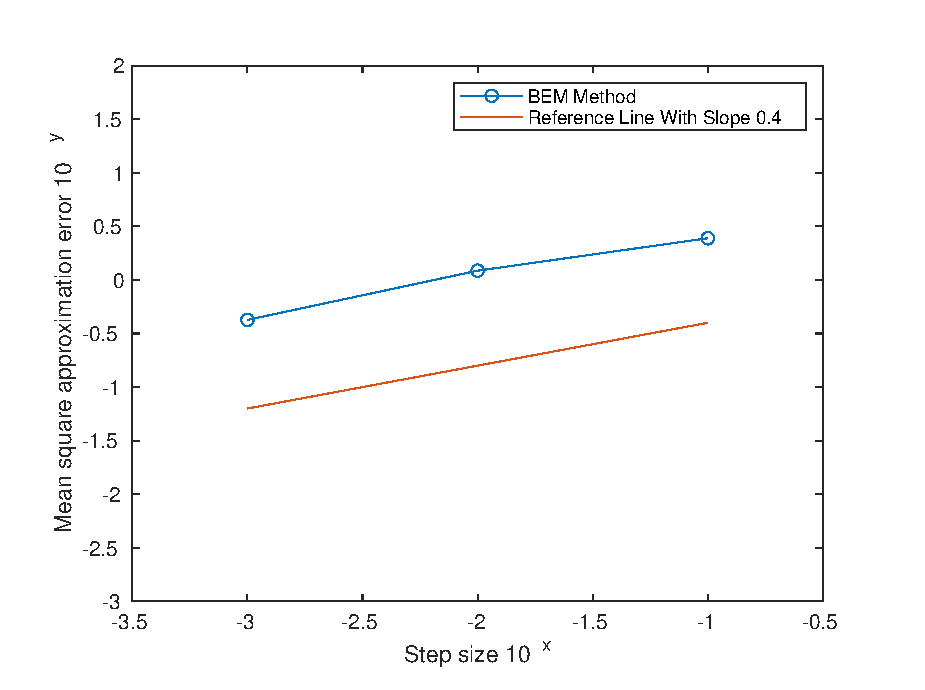
\includegraphics[width=0.45\linewidth]{alpha=0.4.eps}
	\hfill
	\includegraphics[width=0.45\linewidth]{alpha=0.8.eps}
	\caption{EM方法的$L_1$误差, 左图为$\alpha=0.4$, 右图为$\alpha=0.8$}
	\label{fig:image}
	\vspace{-2ex}
	{}\end{figure}